% !TEX root=ManualTFG.tex

\chapter{Information capture}
If we want to play on the Switch, a system that allows us to decrypt what is on screen, to feed it to the neural net is needed. Our first approach was to use some sort of video device, like a webcam, to record what was on screen while simultaneously sending that information to the \ac{PC}. That idea was quickly scrapped, as using a normal capture card was the obvious easiest go to. Thanks to that, we can use Opencv (see more in \ref{appendix:opencv}) to get the images directly in real time with minimal delay in order to perform whichever operations we need to. OpenCV was chosen as our image processing tool mainly because of its vast number of examples and information regarding it.

\section{Detection}
As previously mentioned, a game of Tetris 99 looks like the image in \ref{fig:highlighted}:
 
\begin{figure}[h]
\centering
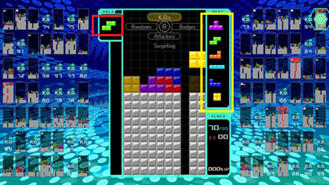
\includegraphics{image003}
\caption{\label{fig:highlighted}Highlighted detection areas}
\end{figure}

Given that the most important information we need is what are the pieces currently in play, a method to detect whether there is one and which type it is had to be devised. At first it was thought this could be guessed by the piece’s own shape but, given rotations and having access to the colour channel, a detection by the later method was much faster and easier to do. Thus, came the idea of calculating the mean colour of each shape in a $5\times 5$ matrix from its center point, including empty blocks and grey pieces. Still, as seen in the previous image, when a piece is placed, it turns a darker tone of its former colour, making us have to factor those in. Thanks to this minor inconvenience, we will later be able to distinguish the main piece from an already placed one if we need to do so. Finally, a small leeway to the mean colour of each piece had to be taken into account when checking for matches due to other elements in the game board influencing the colour of the own piece with shines or shades.

The information we get is also presented back to the user in real time by drawing the conclusions on top of the processed frame. This helps us understand what is being detected and therefore being fed to the neural net. Depending on the detection a string matching the detection will be shown:

\begin{itemize}
	\item	"e": Means empty block.
	\item	"S", "Z", "I", "T", "J", "L", "O": Refers to each of the possible pieces found in a tetris game.
	\item	"gr": Means grey block.
\end{itemize}

There is one more element that will not be shown as a letter, "No match", which will be displayed using the last letter found in the block in white, otherwise their respective piece colour or black for the empty will be shown.

\subsection{Game grid}
The first element we try to detect is the game grid. It can be done thanks to having manually found where the cells center pixel is, and how wide and tall each cell is. By applying a for loop, we can then iterate through each cell and store the information in two arrays with the size of the game grid ($10\times 20$). The first array contains 0's for empty cells, 1's for blocks and 2's for the main piece (game\_matrix), while the second one contains information related to the  colour, including a “no match” variable (info\_matrix). On each iteration, game\_matrix block will be updated only if a match was found, else it will assume the board’s state has not changed.

\subsection{Out of the grid}
The next element we detect is a line upwards out of the main game matrix (row 21). This must be done due to the main piece spawn position going up when it cannot be placed at a certain height, the maximum being 21. This was done separately due to the background colour not being black and because only the main piece is displayed at that height, with placed blocks being hidden by the borders \ref{mainout}, \ref{blocksout}.

%\subsubsection{Main piece out of grid}
\begin{figure}[h]
\centering
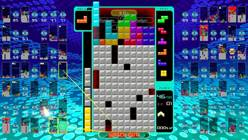
\includegraphics{image020}
\caption{\label{mainout}Main piece out of grid}
\end{figure}

%\subsubsection{Blocks out of grid}
\begin{figure}[h]
\centering
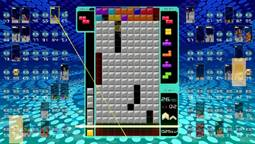
\includegraphics{image021}
\caption{\label{blocksout}Blocks out of grid}
\end{figure}

\subsection{Check stored piece}
To detect which piece (or if none) is in storage, a system that casts two rows of three detection points was built. Each one of those points corresponds to a possible place of a block and, in case it is filled, it updates two matrices with the same system that was built for the game grid detection.

\subsection{Check upcoming pieces}
In order to know what is coming up next, we reused the system to detect stored pieces, this time iterating through a for loop once for each of the upcoming six pieces. Each of the matrices detected is then stored in an array in the same order they are detected (top to bottom).

\section{How noise affects detection}
As mentioned before, we cannot differentiate piece colours without adding a small margin of error for the detection to be consistent in the majority of cases. Unfortunately not only are the colours influenced by other elements, but also visual effects spawn all across the game board depending on the actions done.

To begin with, there is an effect that tells us where our piece is going to be placed (see figure \ref{effects}). Luckily this feature was found to be able to be turned off in the game options, although it is the only one that can be filtered out this easily.

As for the other effects, things like red screen borders, arrows pointing other players and glitter when dropping a piece or sending grey blocks to opponents can also be found interfering with detections (some also seen in \ref{effects}). Many of those directly block what is behind them, so no image processing or margin can be set to minimize or eliminate the obstruction. The best solution we came across is not updating the board information whenever a foreign object is detected, which ends up working pretty well as many of the effects disappear pretty quickly.

\begin{figure}[h]
\centering
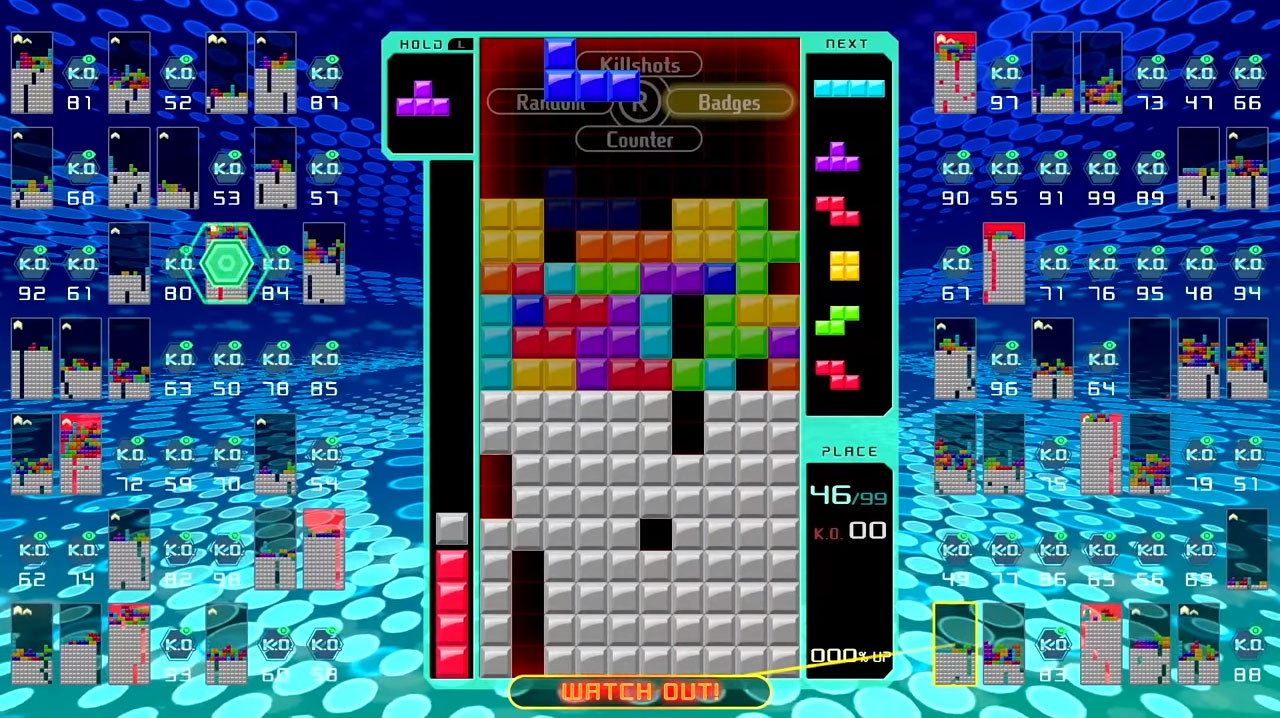
\includegraphics[width=.8\linewidth]{image023}
\caption{\label{effects}Game effects}
\end{figure}

\section{Information adaptation for the neural net}
Once all the information needed has been collected, a way of adapting it so that the neural net understands it had to be made. To do so, we had to convert the data into a Board object of our own Tetris game, with the same configuration detected.

As our neural net works by finding the best combination of consecutive rotations and horizontal movement, and then dropping the piece, we only need to ask for the neural net’s response once (when the piece just spawned). This way we only try to detect new information when the last sequence of movements is completed and when a new piece is detected at the top five rows of the grid, which are the only rows a piece can spawn in plus two more, in case there is a late detection.

When a new main piece is detected, which as mentioned before can be done thanks to it being able to be told apart from the rest because of being slightly brighter, we construct a Piece object with its type and position. The type can easily be guessed by just checking the first blocks's colour but the position is trickier. As all pieces always spawn in the same exact rotation and x position, we can always assign it to be the same, "4", as for the height, we it will be the one of the first block found -1, given that each piece's center block is always one row down except for the "I" piece.

We can now proceed with the creation of the game grid that will be added to the Board object. It is quite simple to do so given that we have a $10\times 20$ array stored with information regarding each cell. We now only have to filter out the main piece, add four empty rows at the top and reverse it to match the object’s model. The actual colour of the placed blocks does not matter, as it is merely an aesthetic element.

Finally, we check if there is a stored piece. If positive, we must then check its colour to know if it is an option for it to be placed or not. That information is then passed on to the Board object.

